Den tredje og sidste metode til at komprimere et stykke tekst med Huffman coding er den adaptive metode. Med den adaptive metode starter træet med at intialisere forekomsten af tegn som de kommer til 1. Når det samme tegn fremkommer igen så vil det blive lagt til tegnets fremkomst værdi, og træet vil derefter også opdatere sig selv sådan hvis et nyt tegn begynder at have flest forekomster så vil den blive placeret øverst i træet. I figur \ref{fig:adaptive_tree} kan man se hvordan det adaptive træ initialisere nye tegn træet støder på til en, og har altid en kontrol knude, N, hvis der skulle komme yderligere nye tegn.

\begin{figure}[H]
\centering
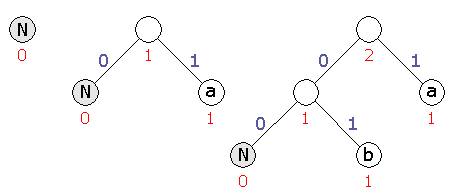
\includegraphics[width=\linewidth]{Billeder/adaptivt.png}
\caption{Initialisering af tegn i et adaptivt træ \cite{Hufftree_1}}
\label{fig:adaptive_tree}
\end{figure}

I forhold til den foregående metode så kan den adaptive metode genere et træ alt efter hvad for noget data som skal komprimeres, ligesom den dynamiske metode, men har til gengæld ikke behov for at videregive en tabel som viser hvordan man oversætter det komprimerede tekst, idet at det adaptive træ på den enhed som dekomprimere vil gøre arbejdet og opdatere sig selv med det data den dekomprimere. Dette kan også betyde at det dynamiske træ muligvis ikke behøver at sende en tabel med over hvis dekomprimeringen sker ved hjælp af det adaptive træ. Ulempen ved den adaptive metode er at det stykke tekst der bliver komprimeret eller dekomprimeret ikke indgår i den nuværende version af træet, idet at det adaptive træ først opdateres med data fra tekststykket efter det er blevet komprimeret eller dekomprimeret. Derudover så kræver den også meget regnekraft fra den enhed som skal komprimere og dekomprimere fordi den konstant skal opdateres af det data den gennemarbejder. \cite{Hufftree_5}

I forhold til SMS beskeder så er den adaptive metoder sikkert bedst når det kommer til at formindske den mængde data der bliver sendt med beskeden. Ulempen er dog at træet har brug for tid til at komme op og køre ved at konstant opdatering af sit eget træ. Den adaptive metode starter derfor ud med at være langsom og ineffektivt idet at den introducere alle tegn fra bunden af og kan først effektivt komprimere efter den har arbejdet sig igennem et antal tekststykker. Kravet for regnekraft på enhederne der komprimere og dekomprimere kan også være en større ulempe på en mobiltelefon.
